%% IEEE TAES manuscript wrapper based on the TAES template.
\PassOptionsToPackage{hypertexnames=false}{hyperref}
\documentclass{IEEEtaes}

\usepackage{amsthm}
\usepackage{amsmath}
\usepackage{amssymb}
\usepackage{amsfonts}
\usepackage{array}
\usepackage{booktabs}
\usepackage{float}
\usepackage{graphicx}
\usepackage{tabularx}
\usepackage{textcomp}
\usepackage[urlcolor=blue,linkcolor=blue,citecolor=blue]{hyperref}
\usepackage{algorithm}
\usepackage{algpseudocode}
\usepackage{cite}

\makeatletter
\setlength{\@fptop}{0pt}
\setlength{\@fpsep}{12pt}
\setlength{\@dblfptop}{0pt}
\setlength{\@dblfpsep}{12pt}
\makeatother

\newcommand{\R}{\mathbb{R}}
\newcommand{\dt}{\Delta t}
\newcommand{\norm}[1]{\left\lVert #1 \right\rVert}
\newcommand{\los}{\mathrm{LOS}}
\newcommand{\fov}{\mathrm{FOV}}
\newcommand{\dv}{\Delta v}
\newcommand{\unit}[2]{#1~#2}

\newtheorem{theorem}{Theorem}
\newtheorem{proposition}{Proposition}
\theoremstyle{remark}
\newtheorem{remark}{Remark}
\theoremstyle{plain}

\begin{document}

\title{Safety-Shielded Candidate-Graph Policy Improvement for Dynamics-Aware Orbital Inspection}

\author{Rugang Tang}
\affil{Northwestern Polytechnical University, Xi'an, China\\ Hong Kong Polytechnic University, Hong Kong, China}

\author{Xin Ning}
\affil{Northwestern Polytechnical University, Xi'an, China}

\author{Chih-Yung Wen}
\affil{Hong Kong Polytechnic University, Hong Kong, China}


\receiveddate{This research was supported, in part by Research Centre of Unmanned Autonomous Systems, Hong Kong Polytechnic University under Grant P0046487.}


\corresp{{\itshape (Corresponding author: Rugang Tang)}.}

\editor{}
\supplementary{Color versions of one or more of the figures in this article are available online at \href{http://ieeexplore.ieee.org}{http://ieeexplore.ieee.org}.}
\markboth{OrbInspect}{Safety-Shielded Orbital Inspection}

\maketitle

\begin{abstract}
Autonomous orbital inspection requires a planner to couple which surface regions are observable with whether consecutive observations are dynamically reachable and auditable. We formulate this problem on a directed candidate graph whose observation nodes store fixed camera-valid masks and whose safe observable orbital arc (SOOA) edges store source-dependent finite-duration Hill--Clohessy--Wiltshire transfers and sampled audit evidence. The main contribution is a set of guarantees for this finite abstraction. We prove that weighted fixed-mask coverage is normalized, monotone, and submodular; that the current node, covered-target and selected-observation masks, and remaining horizon form a sufficient Markov state; and that per-edge input, speed, clearance, terminal, and passive-drift audits are preserved under exact rest-to-rest concatenation at their stored samples. We further prove that final comparison with a feasible incumbent prevents degradation in the shared graph objective, establish a conditional $2H\epsilon$ loss bound for greedy use of a uniformly accurate finite-horizon critic, and show that exhaustive Bellman recursion is optimal on any fixed reduced graph. A safety shield, critic-guided lookahead, rollout, and audited reversal search implement these results. On an ISS mesh, the returned policy preserves 98.33\% coverage while reducing cumulative $\Delta v$ by 9.85\% and three SOOAs relative to the feasible incumbent; ablation attributes this gain to safeguarded local search rather than the critic. The guarantees apply to the deterministic sampled graph and do not imply continuous-time safety or continuous-space optimality.
\end{abstract}

\begin{IEEEkeywords}
spacecraft inspection, approximate dynamic programming, policy iteration, safe observable orbital arc, relative orbital dynamics, passive safety, coverage planning, Hill--Clohessy--Wiltshire equations
\end{IEEEkeywords}

\section{Introduction}
\label{sec:introduction}

Large orbital structures are increasingly important to crewed flight, science, logistics, and in-space assembly. Their external surfaces must be inspected for configuration changes, impact damage, degraded thermal protection, docking-interface anomalies, and other faults that fixed onboard cameras may not observe. An autonomous inspector must therefore decide both where to look and how to move. These decisions are tightly coupled in orbit because a camera pose with high geometric coverage can be unreachable, control-intensive, or unsafe under relative motion.

Existing planning abstractions often expose only one side of this coupling. Robotic next-best-view methods provide mature treatments of sensor range, occlusion, incidence angle, and marginal coverage, but their motion cost is frequently Euclidean or platform-specific. Relative-orbit design provides dynamically meaningful trajectories, yet surface coverage and camera dwell are often secondary constraints rather than the planning objective. A sequential pipeline that selects views first and checks transfers afterward can therefore overestimate useful coverage. The selected views may be attractive in isolation while the connecting trajectory violates input or keep-out limits.

The deeper issue is the definition of a selectable inspection action. A static viewpoint is incomplete because it contains no evidence that the spacecraft can reach that pose under its relative dynamics. A dynamically natural orbit segment is also incomplete when it does not reveal new weighted surface area. For orbital inspection, the action itself should include the transfer, the stabilized camera observation, and the safety evidence used to admit that action. This requirement motivates a finite representation that binds observability and relative-motion feasibility before the coverage sequence is optimized.

We introduce the safe observable orbital arc (SOOA), a source-dependent finite-duration HCW transfer from the current graph node to a stabilized candidate observation. Each SOOA references its destination's camera-valid target set and stores control effort, minimum sampled clearance, terminal error, input and speed status, and optional passive-drift audit. Geometric viewpoints define graph nodes, but they do not contribute coverage until the corresponding directed SOOA has passed the enabled feasibility tests. Figure~\ref{fig:sooa-framework} summarizes the progression from mesh targets and camera visibility to a directed graph of admissible inspection actions. The graph objective then trades newly covered weighted area against the cost of each reachable arc.

The finite representation makes sequential optimization and verification explicit. Candidate nodes are decision nodes, but a node identifier alone is not Markov because the value of a view depends on what has already been covered and how much budget remains. We therefore augment the graph state with covered- and selected-set masks and apply safety-shielded candidate-graph policy improvement. A learned critic, finite lookahead, rollout, and local search generate alternatives, while an audited base policy supplies a feasible completion and a no-degradation safeguard. Exact dynamic programming remains available only for reduced graphs small enough to exhaust.

The contributions are:
\begin{enumerate}
  \item a node--edge representation in which candidate observations store camera-valid target sets and directed SOOAs store source-dependent HCW motion and sampled audit evidence;
  \item a Markov candidate-node formulation and safety-shielded policy-improvement algorithm combining a learned linear critic, truncated Bellman lookahead, incumbent rollout, and audited local search;
  \item proofs of Markov sufficiency, compositional preservation of stored audits, graph-objective incumbent no-degradation, a conditional finite-horizon approximation bound, and exact optimality on exhausted reduced graphs;
  \item matched component, primary, exact-oracle, initial-condition, and compute studies that isolate critic, rollout, safeguard, and local-search contributions and expose their planning-time costs; and
  \item a traceable separation between simulation and visualization in which the experiment writes archived data once and each paper figure is regenerated by a dedicated plotting function.
\end{enumerate}

\begin{figure*}[t]
  \centering
  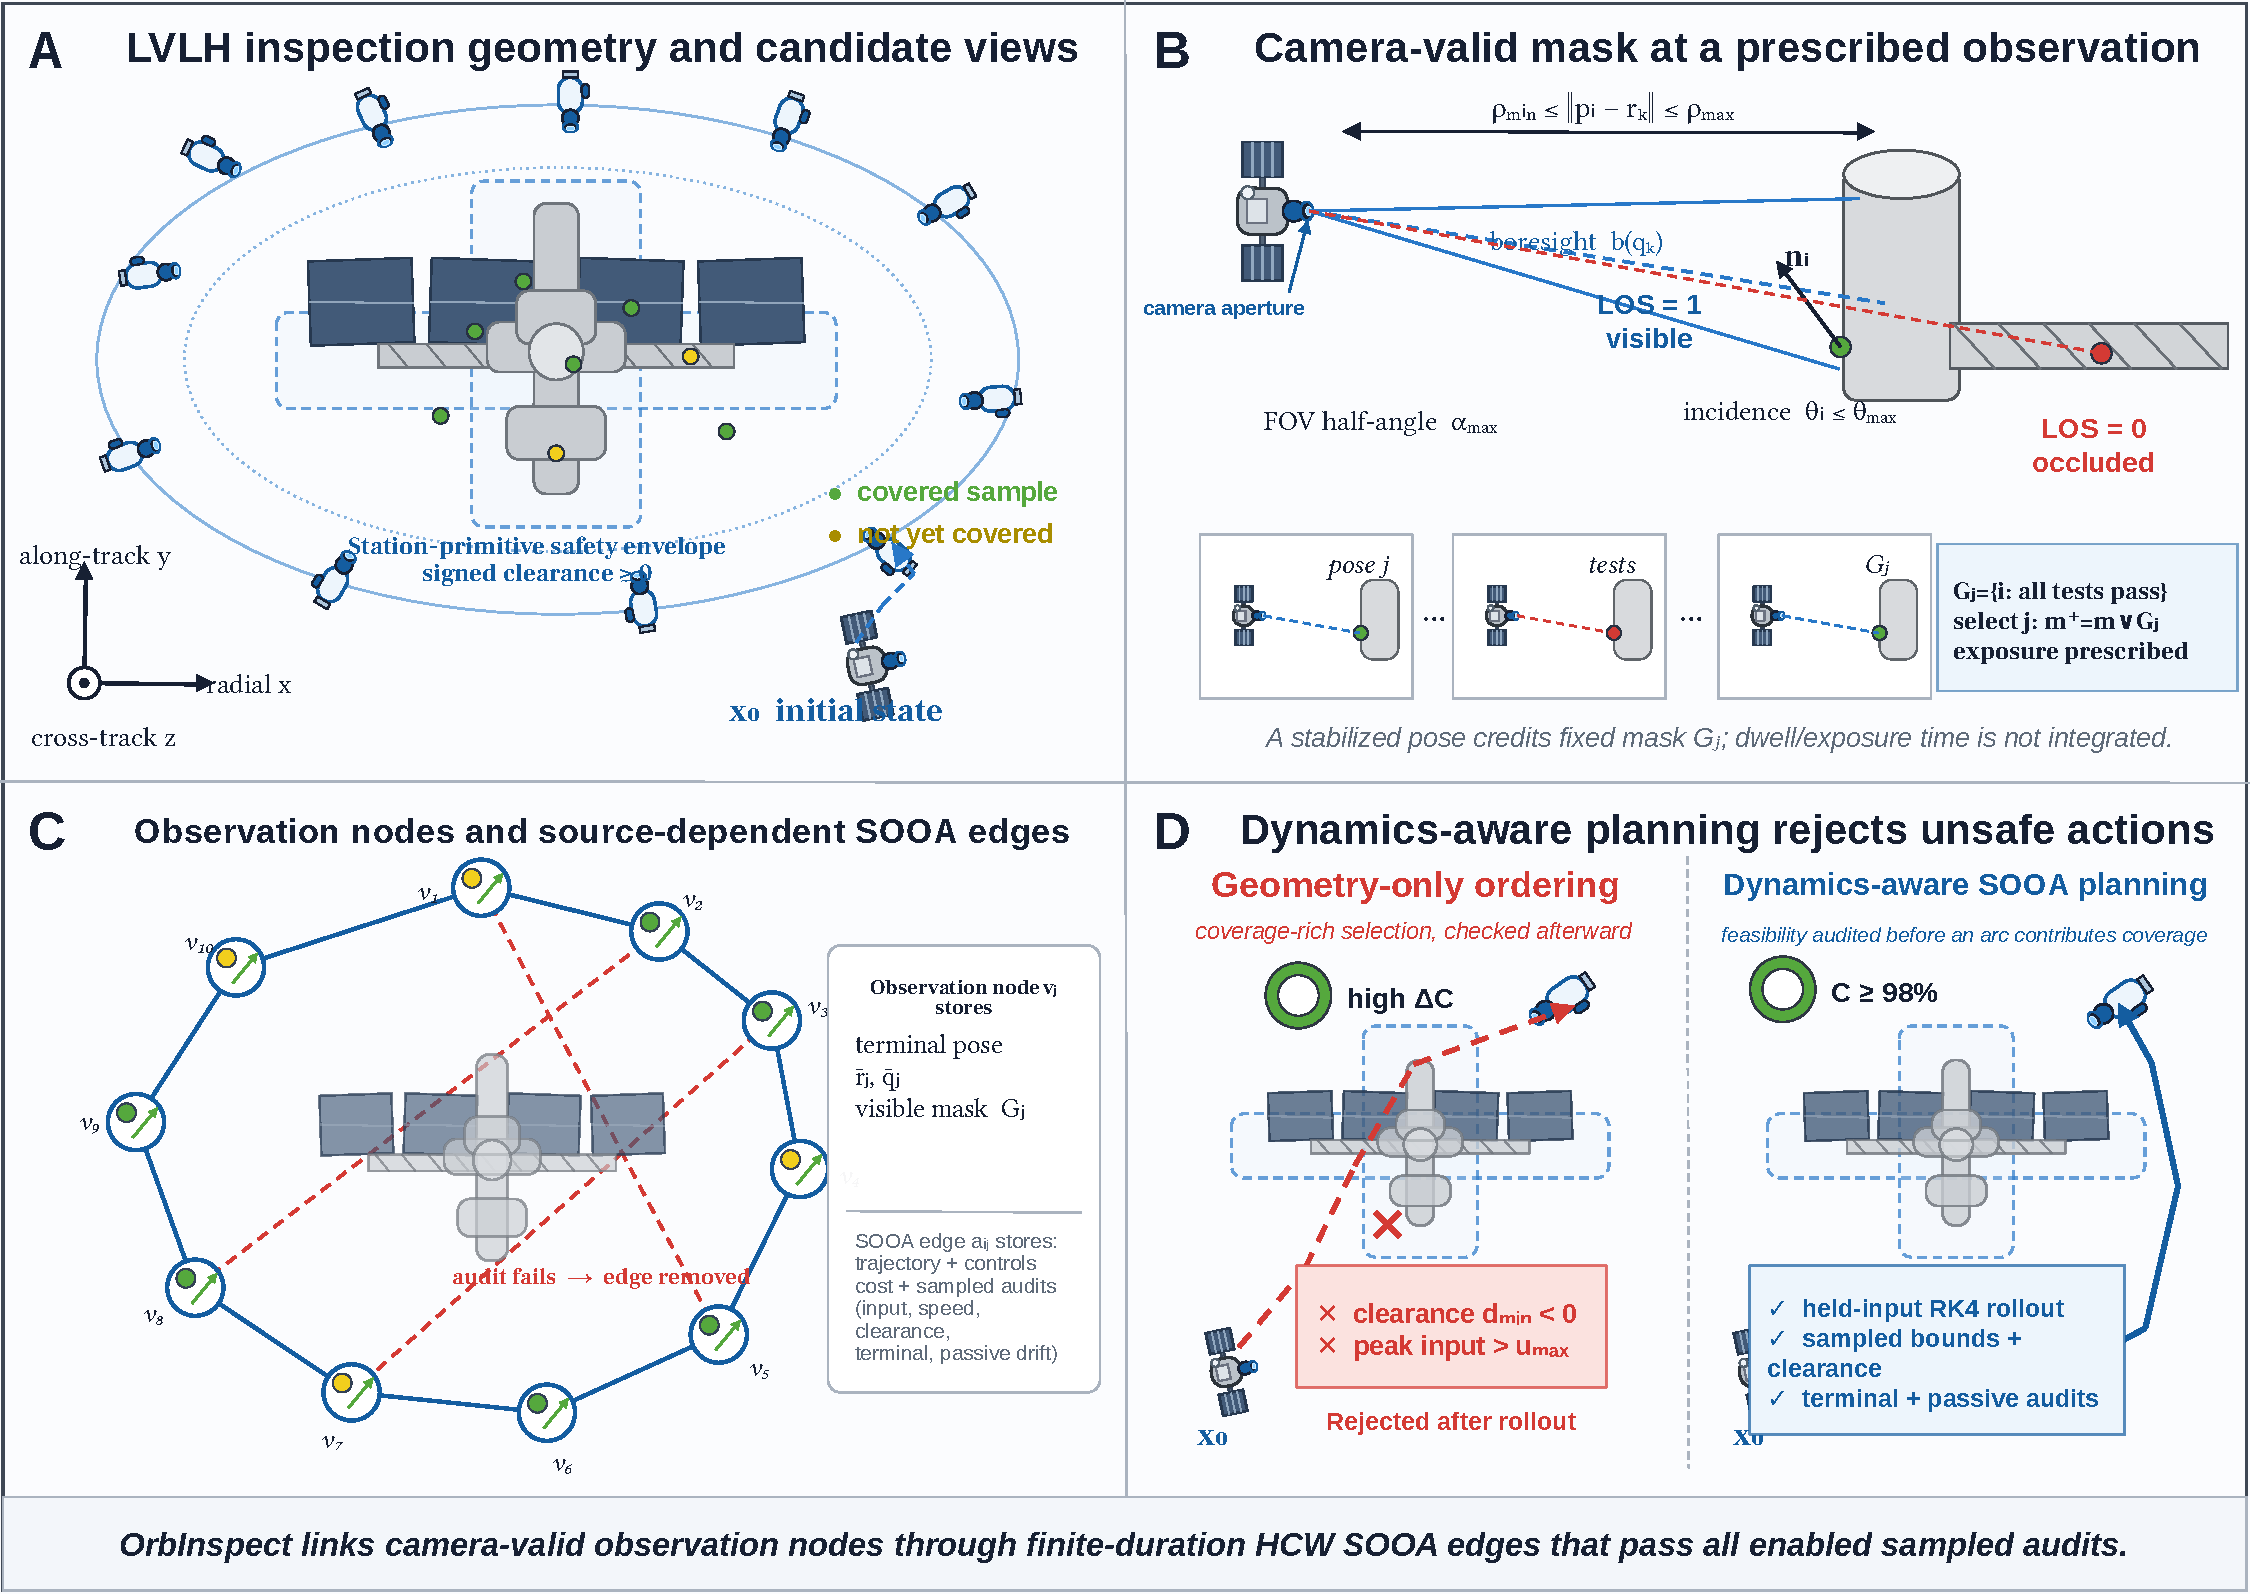
\includegraphics[width=\textwidth]{figures/orbinspect_sooa_framework_editable_revised.pdf}
  \caption{OrbInspect formulation. (a) Candidate observations are generated around an ISS-scale structure and outside a station-primitive safety envelope. (b) Range, field of view, incidence, line of sight, and the prescribed observation condition determine each node's visible-target set. (c) A directed SOOA edge binds a source-dependent HCW transfer and its sampled audits to a destination observation. (d) The graph policy excludes coverage-rich choices whose incoming edge violates an enabled audit.}
  \label{fig:sooa-framework}
\end{figure*}

\section{Related Work}
\label{sec:related}

Relative-motion models provide the dynamic foundation for orbital inspection. The Clohessy--Wiltshire equations remain a common baseline near a circular chief orbit because they are linear, interpretable, and inexpensive to propagate \cite{clohessy1960terminal,wertz2011space}. Higher-fidelity flight design must account for nonlinear gravity, perturbations, navigation error, and actuator dynamics, but HCW propagation is useful for isolating how view ordering changes control effort and safety under a fixed model. Visibility-constrained orbit design has also been studied directly. Hou et al. analyze relative orbits for visual inspection of the China Space Station \cite{hou2024relative}, while Zhou et al. combine near-natural relative ellipses with formation control around a rotating station model \cite{zhou2026formation}. These approaches provide structured orbital motion and stronger closed-loop control analysis than the present planner, but their primary object is an orbit or formation rather than a sequence of surface-coverage actions.

Robotic inspection provides the complementary view-selection perspective. Classical next-best-view work models sensor range, incidence, occlusion, reconstruction quality, and motion cost \cite{scott2003view}. Sampling-based kinodynamic planners such as RRT and asymptotically optimal variants incorporate differential constraints and collision avoidance in continuous state space \cite{lavalle1998rapidly,karaman2011sampling}. These methods are valuable when online reachability or continuous obstacle avoidance dominates. However, surface inspection additionally requires persistent accounting of which weighted targets have satisfied visibility and dwell. That reward must be attached to the motion primitive or repeatedly recomputed during search.

Approximate dynamic programming addresses sequential decisions when exact Bellman recursion is too large. Rollout evaluates a candidate action by completing it with a base policy and can inherit a policy-improvement guarantee in deterministic finite-horizon problems \cite{bertsekas2020rollout,bertsekas1996neuro}. Learning-based policies nevertheless require a separate safety argument: constrained policy optimization controls expected constraint costs \cite{achiam2017cpo}, whereas shielding removes actions that violate an independently specified safety model \cite{alshiekh2018shielding}. OrbInspect uses the latter separation. Learning ranks only candidate actions that have passed a model-based HCW, input, clearance, terminal, and passive-drift audit; it is not trusted to infer safety from a scalar penalty.

Recent spacecraft-inspection studies increasingly couple geometry and motion. Apodaca et al. address inspection trajectory generation and coverage--energy trade-offs for in-orbit structures \cite{apodaca2025trajectory}. Zhou et al. study surface-aware tomographic paths around complex spacecraft geometry \cite{zhou2026tomographic}. Ogri et al. address an execution-level problem involving image-feature tracking, information gain, and dwell under switched-system logic \cite{ogri2025switched}. Together, these studies show that geometric coverage, orbital dynamics, and online sensing cannot be treated as fully independent. They also differ in the level at which the coupling occurs: orbit design, continuous path generation, online camera control, or discrete inspection planning.

OrbInspect is positioned at the discrete-action level. Its contribution is neither a new relative dynamics model nor a flight-certified collision-avoidance controller. Each SOOA is simultaneously a sensor-valid coverage contributor and a dynamically audited finite motion, so an infeasible transfer cannot improve the planner's reported coverage. This representation gives more detailed camera and sequential view-selection logic than formation-level observation studies, while those studies provide lessons for future work: near-natural relative arcs can seed lower-effort SOOA libraries, and a rotating body frame should replace the fixed-LVLH target assumption when station attitude motion is material. The current optimality claim remains conditional on the sampled library, and continuous-space global optimality is outside scope.

\section{System and Observation Model}
\label{sec:system}

The present study addresses offline planning. It receives a known station mesh, an initial relative state, camera parameters, a keep-out model, and actuation limits, and returns a time-indexed translational reference, a camera-boresight stream, selected SOOA records, and summary metrics. A future ROS~2 replay layer may publish these records, but no ROS or Gazebo result is used to support the quantitative claims in this manuscript.

\begin{table*}[t]
  \centering
  \caption{Modeling assumptions and the boundary of the reported evidence.}
  \label{tab:assumptions}
  \renewcommand{\arraystretch}{1.08}
  \setlength{\tabcolsep}{5pt}
  \footnotesize
  \begin{tabularx}{\textwidth}{@{}p{0.18\textwidth}p{0.34\textwidth}X@{}}
    \toprule
    Assumption & Role in the baseline & Consequence for interpretation \\
    \midrule
    Circular chief orbit & Supports linear HCW relative translation in the LVLH frame. & Quantitative results compare planners under the same local linear model, not a perturbed flight ephemeris. \\
    Station fixed in LVLH & Keeps mesh targets and safety primitives stationary during one planning run. & Rotating appendages or station attitude motion require a body-frame extension. \\
    Known mesh and state & Makes visibility, occlusion, and transfer evaluation deterministic. & Navigation, map, and shape uncertainty are not represented by the present safety margin. \\
    Prescribed camera attitude & Points the boresight toward each candidate observation target and exports the corresponding quaternion stream. & Camera slew time, reaction-wheel limits, and closed-loop attitude error are outside the optimization. \\
    Sampled safety envelope & Computes signed clearance to station primitives at every rollout sample. & Positive sampled clearance is a planning audit rather than a continuous-time collision certificate. \\
    No illumination or plume model & Isolates view geometry and translational feasibility. & Sun angle, shadow, contamination, and plume-impingement restrictions must be added for flight design. \\
    \bottomrule
  \end{tabularx}
\end{table*}

\subsection{Relative Dynamics}

The inspected structure is fixed in an LVLH frame attached to a nominal circular chief orbit. The axes follow the radial, along-track, and cross-track directions shown in Fig.~\ref{fig:sooa-framework}. The chaser state is $\mathbf{x}=[\mathbf{r}^{\mathsf T},\mathbf{v}^{\mathsf T}]^{\mathsf T}\in\R^6$, where $\mathbf r=[r_x,r_y,r_z]^{\mathsf T}$ and $\mathbf v=[v_x,v_y,v_z]^{\mathsf T}$. With mean motion $n$ and commanded acceleration $\mathbf{u}=[a_x,a_y,a_z]^{\mathsf T}$, the HCW model is
\begin{equation}
  \begin{aligned}
  \dot{\mathbf{x}}&=A_{\mathrm{HCW}}\mathbf{x}+B\mathbf{u},\\
  A_{\mathrm{HCW}}&=\begin{bmatrix}0&I\\K_n&C_n\end{bmatrix},
  &B&=\begin{bmatrix}0\\I\end{bmatrix},\\
  K_n&=\operatorname{diag}(3n^2,0,-n^2),
  &C_n&=\begin{bmatrix}0&2n&0\\-2n&0&0\\0&0&0\end{bmatrix}.
  \end{aligned}
  \label{eq:hcw-continuous}
\end{equation}
For the continuous HCW model, piecewise-constant acceleration over $\dt$ has the exact zero-order-hold map
\begin{equation}
  \begin{aligned}
  \mathbf{x}_{k+1}&=A_d\mathbf{x}_k+B_d\mathbf{u}_k,\\
  A_d&=e^{A_{\mathrm{HCW}}\dt},\\
  B_d&=\int_0^{\dt}e^{A_{\mathrm{HCW}}\tau}B\,d\tau.
  \end{aligned}
  \label{eq:hcw-discrete}
\end{equation}
The reported implementation uses the same piecewise-constant input model but constructs and propagates each discrete boundary map with fixed-step fourth-order Runge--Kutta integration. We denote that numerical affine map by $\mathbf x_{k+1}=\widetilde A_d\mathbf x_k+\widetilde B_d\mathbf u_k$; Eq.~\eqref{eq:hcw-discrete} is the exact continuous-model reference, not a claim that the archived samples were generated by a matrix exponential. The transfer is therefore a finite-duration continuous-thrust maneuver with zero-order-held acceleration, which may jump at sample boundaries, rather than an impulsive maneuver. Each segment is solved rest-to-rest at a candidate observation, and the numerical rollout is accepted only when its terminal position and velocity errors satisfy the stated tolerances.

\subsection{Visibility, Prescribed Observation, and Coverage}

The structure is represented by weighted surface samples $\mathcal T=\{(p_i,n_i,w_i)\}_{i=1}^{N}$ with $w_i>0$. Each weight approximates the surface area represented by its sample, so a densely tessellated component does not dominate solely because it contains more vertices. The camera attitude $q_k$ defines unit boresight $b(q_k)$, and $\mathcal O$ denotes the occluding mesh. Target $i$ is visible when
\begin{align}
  r_{\min}^{\mathrm{cam}}&\le\norm{p_i-\mathbf r_k}\le r_{\max}^{\mathrm{cam}},\nonumber\\
  \arccos\!\frac{(p_i-\mathbf r_k)^{\mathsf T}b(q_k)}
  {\norm{p_i-\mathbf r_k}}&\le\alpha_{\max},\nonumber\\
  \arccos\!\frac{(\mathbf r_k-p_i)^{\mathsf T}n_i}
  {\norm{\mathbf r_k-p_i}\norm{n_i}}&\le\theta_{\max},\nonumber\\
  \los(\mathbf r_k,p_i,\mathcal O)&=1.
  \label{eq:visibility}
\end{align}
The four tests exclude targets that are too near or too far, outside the field of view, observed at an excessive incidence angle, or blocked by station geometry. In a closed-loop execution model, dwell could be accumulated as $\tau_{i,k+1}=\tau_{i,k}+\dt$ while target $i$ remains visible and accepted when $\tau_i\ge\tau_{\min}$. The archived offline study instead treats every candidate as a stabilized terminal observation with its prescribed exposure completed a priori. Selecting node $j$ therefore credits its fixed visibility mask $G_j$, so $m_{k+1}=m_k\lor G_j$. The weighted coverage represented by mask $m_k$ is
\begin{equation}
  C(m_k)=\frac{\sum_i w_i m_{i,k}}{\sum_i w_i}.
  \label{eq:coverage}
\end{equation}

Candidate generation can make a subset of the sampled surface invisible from every candidate observation. For the nonempty set $\mathcal T_{\mathrm{insp}}=\cup_{j=1}^{M}G_j$, we therefore also report inspectable coverage:
\begin{equation}
  C_k^{\mathrm{insp}}=
  \frac{\sum_{i\in\mathcal T_{\mathrm{insp}}}w_i m_{i,k}}
  {\sum_{i\in\mathcal T_{\mathrm{insp}}}w_i}.
  \label{eq:inspectable-coverage}
\end{equation}
The total coverage in Eq.~\eqref{eq:coverage} measures how much of the sampled structure is credited, whereas Eq.~\eqref{eq:inspectable-coverage} conditions on the candidate library. The reported mission duration includes transfer time but no additional dwell or exposure time. Attitude determines the visibility predicate and exported boresight; closed-loop attitude dynamics, illumination, and interruption of a dwell are outside the offline model.

\subsection{Dynamic Feasibility and SOOAs}

Every sampled state must satisfy
\begin{equation}
  \norm{\mathbf u_k}_2\le u_{\max},\qquad
  \norm{\mathbf v_k}_2\le v_{\max},\qquad
  d_{\mathcal S}(\mathbf r_k)\ge 0,
  \label{eq:limits}
\end{equation}
where $d_{\mathcal S}(\mathbf r)=d_{\mathrm{surf}}(\mathbf r)-d_{\mathrm{safe}}$ is signed clearance above the already inflated keep-out margin; thus $d_{\mathcal S}=0$ is the admissibility boundary. For a directed rollout from source node $i$ to destination node $j$, define $\Delta v_{ij}=\sum_k\norm{\mathbf u_{ij,k}}_2\dt$, root-mean-square distance $e_{ij}^{\mathrm{rms}}$ from the transfer samples to the destination position, and $d_{ij}^{\min}=\min_k d_{\mathcal S}(\mathbf r_{ij,k})$. The graph stage cost used in the reported study is
\begin{equation}
  \ell_{ij}=\lambda_v\Delta v_{ij}+\lambda_e e_{ij}^{\mathrm{rms}}+\lambda_s\max(0,-d_{ij}^{\min})+\lambda_a.
  \label{eq:edge-cost}
\end{equation}
For every shield-admissible edge, the clearance-violation term is zero. It remains in the shared cost implementation so deliberately unshielded comparison methods can be evaluated with the same expression.

A candidate observation node and a directed SOOA edge are, respectively,
\begin{equation}
  \begin{aligned}
  v_j&=(\bar{\mathbf r}_j,\bar q_j,G_j),\\
  a_{ij}&=\bigl(\mathbf x_{ij}[1{:}K],\mathbf u_{ij}[0{:}K-1],q_{ij}[1{:}K],\\
  &\qquad \Delta v_{ij},d_{ij}^{\min},u_{ij}^{\max},v_{ij}^{\max},e_{ij}^{r},e_{ij}^{v},\rho_{ij}\bigr).
  \end{aligned}
  \label{eq:sooa}
\end{equation}
Here $\bar{\mathbf r}_j$ and $\bar q_j$ are the terminal observation pose and prescribed attitude, $G_j\subseteq\mathcal T$ is its camera-valid target set, and $e_{ij}^{r}$ and $e_{ij}^{v}$ are terminal position and velocity errors. The stored state and attitude arrays contain the $K$ post-step samples; the source state is held by node $v_i$. The initial condition is a distinguished source node $v_0$ with no visibility reward. For passive horizon $T_p=L_p\dt$, the optional audit propagates zero-input HCW drift from every stored edge state and records $\rho_{ij}=\min_{1\le k\le K,\,0\le l\le L_p}d_{\mathcal S}(\mathbf r_{ij,k}^{\mathrm{drift}}(l))$. An edge is admitted only when all enabled sampled inequalities and terminal tolerances pass. Throughout this paper, ``safe'' in SOOA means admissible under these enabled sampled audits. Neither $d_{ij}^{\min}\ge0$ nor $\rho_{ij}\ge0$ certifies clearance between integration samples or under model uncertainty.

\section{Safety-Shielded Candidate-Graph Policy Improvement}
\label{sec:algorithm}

\subsection{Candidate Graph and Markov State}

Let $\mathcal V=\{v_0,v_1,\ldots,v_M\}$ contain the initial node and the $M$ candidate observation nodes in Eq.~\eqref{eq:sooa}. A directed edge from $v_i$ to $v_j$ is the source-dependent SOOA $a_{ij}$, and it is absent when an enabled audit fails. Thus visibility $G_j$ is node dependent, whereas trajectory, cost, clearance, input, terminal error, and passive margin are edge dependent. This separation is necessary because reaching the same observation from two different source nodes generally produces different HCW motion and audit values.

A node identifier is not a sufficient decision state because the value of a view changes after its targets have been covered. The finite-horizon Markov state is
\begin{equation}
  s_k=(j_k,m_k,b_k,h_k),
  \label{eq:mdp-state}
\end{equation}
where $j_k\in\{0,\ldots,M\}$ is the current node, $m_k\in\{0,1\}^{N}$ is the covered-target mask, $b_k\in\{0,1\}^{M}$ is the selected-observation mask, and $h_k$ is the remaining action budget. Selecting destination $a\in\{1,\ldots,M\}$ traverses edge $a_{j_ka}$ and gives the deterministic transition
\begin{equation}
  f(s_k,a)=\left(a,\;m_k\lor G_a,\;b_k\lor\mathbf e_a,\;h_k-1\right).
  \label{eq:mdp-transition}
\end{equation}
The shield-admissible action set $\mathcal U_s(s)$ is defined below. The constrained graph problem assigns zero terminal cost after reaching $C_{\mathrm{req}}$ and value $+\infty$ when no goal-reaching continuation exists within the remaining budget. Its Bellman recursion is
\begin{equation}
  \begin{aligned}
  V^\star(s)&=
    \begin{cases}
    0, & C(m)\ge C_{\mathrm{req}},\\
    +\infty, & h=0\ \text{or}\ \mathcal U_s(s)=\varnothing,\\
    \min\limits_{a\in\mathcal U_s(s)}
      Q^\star(s,a), & \text{otherwise},
    \end{cases}\\
  Q^\star(s,a)&=\ell_{j a}+V^\star(f(s,a)).
  \end{aligned}
  \label{eq:bellman}
\end{equation}
Here $j$ and $h$ are the current-node and remaining-budget components of $s$. The infinite value enforces the coverage constraint in the exact oracle; it is not the finite loss used to train the critic.

\subsection{SOOA Construction and Safety Shield}

Area-weighted targets are sampled from the mesh, and camera seeds are generated on offset shells around their outward normals. The binary visibility matrix $V_{ij}=\mathbf 1\{i\in G_j\}$ is computed once from the terminal observation geometry. For a transition to $\bar{\mathbf x}_j=[\bar{\mathbf r}_j^{\mathsf T},\mathbf0^{\mathsf T}]^{\mathsf T}$, the planner solves the minimum-energy piecewise-constant HCW boundary-value problem under the numerical RK4 map
\begin{equation}
  \begin{aligned}
  \min_{\mathbf u_0,\ldots,\mathbf u_{K-1}}\quad&
  \sum_{k=0}^{K-1}\norm{\mathbf u_k}_2^2\\
  \mathrm{s.t.}\quad&
  \mathbf x_{k+1}=\widetilde A_d\mathbf x_k+\widetilde B_d\mathbf u_k,\\
  &\mathbf x_K=\bar{\mathbf x}_j.
  \end{aligned}
  \label{eq:terminal-transfer}
\end{equation}
If the terminal influence matrix $\mathcal B_K=[\widetilde A_d^{K-1}\widetilde B_d\ \cdots\ \widetilde B_d]$ has full row rank, the stacked minimum-norm command from source state $\mathbf x_i^{\mathrm{src}}$ is $\mathbf U_{ij}^\star=\mathcal B_K^{\mathsf T}(\mathcal B_K\mathcal B_K^{\mathsf T})^{-1}(\bar{\mathbf x}_j-\widetilde A_d^K\mathbf x_i^{\mathrm{src}})$. The implementation computes this expression through the $6\times6$ Gram system and then propagates the requested input without clipping. Let $\chi_{ij}=1$ exactly when every stored edge sample satisfies Eq.~\eqref{eq:limits}, $e_{ij}^{r}\le\varepsilon_r$, $e_{ij}^{v}\le\varepsilon_v$, and $\rho_{ij}\ge0$ when the passive audit is enabled. The shield then admits
\begin{equation}
  \mathcal U_s(s)=
  \left\{a\in\{1,\ldots,M\}:\begin{array}{l}b_a=0,\;G_a\setminus m\neq\varnothing,\\\chi_{ja}=1\end{array}\right\},
  \label{eq:safe-action-set}
\end{equation}
where $j$ is the current-node component of $s$. Unlike a reward penalty, the shield makes an inadmissible edge unavailable to critic training, approximate selection, rollout, local search, and exact recursion \cite{alshiekh2018shielding}. The guarantee remains conditional on the sampled numerical rollout and the deterministic model used to compute $\chi_{ij}$.

\subsection{Critic, Lookahead, and Safeguarded Improvement}

Exact recursion is exponential in the coverage and selected-node masks. The approximate planner first screens the largest marginal-coverage candidates, audits at most a configured candidate width, and retains a critic-ranked branch $\mathcal B_w(s)\subseteq\mathcal U_s(s)$. The archived paper study approximates action value by $\widehat Q_w(s,a)=w^{\mathsf T}\phi(s,a)$ with ten normalized features: a bias, post-action coverage gap and its square, stage cost, marginal weighted coverage, coverage-per-cost efficiency, used-budget fraction, inverse remaining horizon, clearance deficit, and input ratio. These ten features define the reported results; changing the feature map requires retraining and constitutes a different experimental configuration.

Critic fitting uses a finite failure loss rather than the infinite constrained value in Eq.~\eqref{eq:bellman}. For any fixed screened action set $\mathcal B(s)\subseteq\mathcal U_s(s)$, define $\Psi(s)=\lambda_C[0.5+(C_{\mathrm{req}}-C(m))/C_{\mathrm{req}}]$ and the finite surrogate recursion
\begin{equation}
  \begin{aligned}
  \widetilde V^\star(s)&=\begin{cases}
  0,&C(m)\ge C_{\mathrm{req}},\\
  \Psi(s),&h=0\ \text{or}\ \mathcal B(s)=\varnothing,\\
  \min\limits_{a\in\mathcal B(s)}\widetilde Q^\star(s,a),&\text{otherwise},
  \end{cases}\\
  \widetilde Q^\star(s,a)&=\ell_{ja}+\widetilde V^\star(f(s,a)).
  \end{aligned}
  \label{eq:critic-surrogate}
\end{equation}
Safe exploratory rollouts generate Monte Carlo returns for this finite-loss objective, and normalized stochastic-gradient updates fit $w$. After training, the online selector freezes the critic, expands a bounded safe branch for $d$ steps, and uses $\widehat Q_w$ at truncated leaves. The critic therefore approximates a screened finite-horizon value calculation; it neither certifies feasibility nor solves the full constrained recursion \cite{bertsekas1996neuro}.

A deterministic two-stage coverage-and-HCW tour supplies a base policy $\mu_0$. One-step rollout evaluates an admissible action by
\begin{equation}
  Q_{\mu_0}(s,a)=\ell_{ja}+J_{\mu_0}\!\left(f(s,a)\right),
  \label{eq:rollout}
\end{equation}
where $J_{\mu_0}$ is obtained by executing the remaining base order through the same shield. Rollout retains an action only when this completion reaches the coverage goal within the remaining budget. Audited reversal moves then search the incumbent sequence, and final selection minimizes the common graph objective over the successful learned, rollout, base, and locally improved candidates. Including a feasible incumbent in this final comparison, rather than trusting predicted partial cost, provides the no-degradation property below.

\begin{algorithm}[t]
\caption{Safety-shielded candidate-graph policy improvement}
\label{alg:safe-graph-api}
\begin{algorithmic}[1]
\Require Candidate nodes, lazy directed-SOOA evaluator, goal $C_{\mathrm{req}}$, budget $H$
\State Build the deterministic feasible base policy $\mu_0$
\State Fit $\widehat Q_w$ from shielded Monte Carlo rollouts
\State Generate $\pi_{\mathrm{C}}$ by depth-$d$ critic-guided finite-loss lookahead
\For{each rollout decision state $s$}
  \State Form shielded critic-ranked actions and remaining base actions
  \State Evaluate Eq.~\eqref{eq:rollout} using audited base completions
  \State Select the minimum-cost action with a feasible completion
\EndFor
\State Audit bounded reversal moves of the base sequence
\State Return the least-cost successful candidate among $\pi_{\mathrm{C}}$, rollout, base, and improved base
\State Export policy source, critic errors, rejected actions, exact gap when available, and all trajectory records
\end{algorithmic}
\end{algorithm}

\subsection{Properties and Exact Oracle}
\label{sec:theory}

\begin{proposition}[Monotone submodularity of fixed-mask coverage]
\label{prop:submodular-coverage}
For an observation set $S\subseteq\{1,\ldots,M\}$, let $F(S)=\sum_{i=1}^{N}w_i\mathbf1\{i\in\cup_{j\in S}G_j\}$. If all $w_i\ge0$, then $F$ is normalized, monotone, and submodular.
\end{proposition}

\begin{IEEEproof}
Clearly $F(\varnothing)=0$. If $A\subseteq B$, every target covered by $A$ is covered by $B$, so nonnegative weights give $F(A)\le F(B)$. For $a\notin B$, the marginal gain $F(A\cup\{a\})-F(A)$ is the total weight in $G_a\setminus\cup_{j\in A}G_j$. Since $A\subseteq B$, this set contains $G_a\setminus\cup_{j\in B}G_j$, proving diminishing returns.
\end{IEEEproof}

\begin{remark}[Role of submodularity]
Proposition~\ref{prop:submodular-coverage} justifies marginal-coverage screening at the node level. It does not supply a greedy approximation ratio for the complete inspection tour because the directed SOOA cost and admissibility of the next observation depend on the current node.
\end{remark}

\begin{proposition}[Markov sufficiency]
\label{prop:markov-sufficiency}
For a fixed deterministic candidate graph with fixed node masks, source-dependent edge records, target weights, revisit rule, and horizon, the state in Eq.~\eqref{eq:mdp-state} is Markov for the finite graph decision problem.
\end{proposition}

\begin{IEEEproof}
The current node $j_k$ identifies the source of every possible next edge; $m_k$ determines marginal and terminal coverage; $b_k$ determines which observations remain selectable under the no-revisit rule; and $h_k$ determines the remaining budget. By assumption, visibility masks and edge costs and audits are deterministic records indexed only by the current and destination nodes. Equations~\eqref{eq:mdp-transition}, \eqref{eq:bellman}, and \eqref{eq:safe-action-set} therefore depend on no earlier history once $(j_k,m_k,b_k,h_k)$ is given. The proposition concerns this finite graph abstraction, not the underlying uncertain continuous spacecraft system.
\end{IEEEproof}

\begin{proposition}[Compositional preservation of stored audits]
\label{prop:audit-composition}
Consider a sequence $(a_{j_{k-1}j_k})_{k=1}^{L}$ whose first source is $v_0$, whose idealized rest-to-rest endpoints match exactly, and whose every edge has $\chi_{j_{k-1}j_k}=1$. Then every stored sample of the concatenated sequence satisfies the input, speed, and clearance inequalities, every edge endpoint satisfies its terminal conditions, and every stored passive-drift rollout has nonnegative margin when that audit is enabled.
\end{proposition}

\begin{IEEEproof}
By the definition of $\chi_{ij}$, all stated conditions hold on each accepted edge record. Exact endpoint matching identifies the terminal state of edge $k$ with the source state of edge $k+1$, so the records concatenate without an unmodelled jump. The sample set of the complete trajectory is the finite union of the per-edge sample sets; therefore every member of that union retains the corresponding per-edge audit result.
\end{IEEEproof}

\begin{remark}[Meaning of audit preservation]
The proposition is a finite-record composition result, not a continuous-time barrier certificate. It does not cover inter-sample clearance, endpoint perturbations beyond tolerance, closed-loop tracking error, or robustness to model and state uncertainty.
\end{remark}

\begin{theorem}[Incumbent no-degradation in the graph objective]
\label{thm:incumbent}
Let $\Pi_{\mathrm{cand}}$ be the finite set compared in the final line of Algorithm~\ref{alg:safe-graph-api}, and let $\Pi_F\subseteq\Pi_{\mathrm{cand}}$ contain exactly the sequences that reach $C_{\mathrm{req}}$ within $H$ actions using only edges in Eq.~\eqref{eq:safe-action-set}. Define $J(\pi)=\sum_{a_{ij}\in\pi}\ell_{ij}$. If the incumbent $\mu_0\in\Pi_F$ and the algorithm returns $\widehat\pi\in\arg\min_{\pi\in\Pi_F}J(\pi)$, then $\widehat\pi$ is graph feasible and $J(\widehat\pi)\le J(\mu_0)$.
\end{theorem}

\begin{IEEEproof}
The assumption $\mu_0\in\Pi_F$ makes the feasible comparison set nonempty. Since $\widehat\pi$ minimizes $J$ over a set that contains $\mu_0$, $J(\widehat\pi)\le J(\mu_0)$, and membership in $\Pi_F$ supplies the stated graph feasibility.
\end{IEEEproof}

\begin{remark}[Scope of the safeguard]
No-degradation concerns the common stage-cost sum and requires a feasible incumbent in the comparison set. It does not imply lower $\Delta v$, shorter runtime, or improvement of any individual metric unless that conclusion is established separately.
\end{remark}

\begin{proposition}[Conditional finite-horizon approximation bound]
\label{prop:critic-bound}
Fix a finite surrogate problem of the form in Eq.~\eqref{eq:critic-surrogate}, including its screened action sets and finite terminal loss, and write $\widetilde Q_h^\star$ and $\widetilde V_h^\star$ for its values at states with $h$ decisions remaining. Suppose $|\widehat Q_h(s,a)-\widetilde Q_h^\star(s,a)|\le\epsilon$ for every reachable nonterminal state, every $a\in\mathcal B(s)$, and every $1\le h\le H$. If $\pi_{\widehat Q}$ selects an action minimizing the matching $\widehat Q_h$, then $J_{\Psi}(\pi_{\widehat Q};s_0)-\widetilde V_H^\star(s_0)\le2H\epsilon$, where $J_{\Psi}$ includes the same finite terminal loss as Eq.~\eqref{eq:critic-surrogate}.
\end{proposition}

\begin{IEEEproof}
At a nonterminal state with $h$ decisions remaining, let $\widehat a$ minimize $\widehat Q_h$ and let $a^\star$ minimize $\widetilde Q_h^\star$. The uniform bound and approximate greediness give $\widetilde Q_h^\star(s,\widehat a)\le\widehat Q_h(s,\widehat a)+\epsilon\le\widehat Q_h(s,a^\star)+\epsilon\le\widetilde Q_h^\star(s,a^\star)+2\epsilon$. Let $D_h(s)=J_{\Psi}(\pi_{\widehat Q};s)-\widetilde V_h^\star(s)$. Stage costs cancel between the actual continuation through $\widehat a$ and $\widetilde Q_h^\star(s,\widehat a)$, so $D_h(s)\le2\epsilon+D_{h-1}(f(s,\widehat a))$. At every goal, zero-budget, or empty-action boundary state, the policy and optimal values use the same terminal loss, so the corresponding difference is zero. Induction yields $D_H(s_0)\le2H\epsilon$.
\end{IEEEproof}

\begin{remark}[Conditional nature of the critic bound]
Proposition~\ref{prop:critic-bound} is a sensitivity result for a fixed finite surrogate problem. The reported experiments do not establish the assumed uniform error bound, so the proposition is neither a critic-convergence theorem nor an empirical performance guarantee, and it does not apply to the infinite failure values in Eq.~\eqref{eq:bellman}.
\end{remark}

For reduced-graph certification, exact recursion caches Eq.~\eqref{eq:bellman} for every reachable tuple $(j,m,b,h)$ and enumerates every action in $\mathcal U_s(s)$ rather than the critic-screened branch.

\begin{theorem}[Optimality on an exhausted reduced SOOA graph]
\label{thm:reduced-optimality}
For fixed finite nodes, deterministic visibility masks, deterministic audited edge costs, a coverage requirement, and horizon $H$, exhaustive evaluation of Eq.~\eqref{eq:bellman} returns a minimum-cost goal-reaching shield-feasible sequence when one exists. If no such sequence exists, it returns value $+\infty$ and reports infeasibility.
\end{theorem}

\begin{IEEEproof}
Proceed by induction on the remaining budget $h$. At $h=0$, Eq.~\eqref{eq:bellman} returns zero exactly for a goal state and $+\infty$ otherwise, which is correct. Assume the recursion is correct for all states with at most $h-1$ remaining actions. At a state with $h$ actions, every feasible sequence begins with exactly one $a\in\mathcal U_s(s)$ and then a feasible continuation from $f(s,a)$; by the induction hypothesis, the recursion assigns that continuation its minimum cost or $+\infty$ if none exists. Minimizing over every admissible first action therefore returns the minimum total cost, or $+\infty$ when all continuations are infeasible. The claim is limited to the exhausted sampled graph and does not extend to omitted camera poses or continuous-space trajectories.
\end{IEEEproof}

\begin{remark}[Graph certificate versus mission optimality]
Theorem~\ref{thm:reduced-optimality} certifies only the nodes, edges, masks, and audits included in the exhausted graph. Omitted camera poses, alternative transfer durations, and continuous-space trajectories remain outside the certified decision set.
\end{remark}

\section{Experimental Protocol}
\label{sec:simulation}

\subsection{Base Benchmark}

The full benchmark uses the public NASA ISS glTF mesh \cite{nasa_iss_gltf_model}. The mesh is transformed into the planner's LVLH convention and sampled into 180 area-weighted targets. Offset-shell generation produces 357 camera candidates at a nominal \unit{34}{m} radius. The initial state is $[0,-35,10,0,0,0]^{\mathsf T}$ in SI units, the HCW mean motion is $1.13137\times10^{-3}$~rad/s, the keep-out margin is \unit{2}{m}, the view budget is 36, and the training seed is 7. Every rest-to-rest segment lasts \unit{90}{s} and uses fixed-step RK4 propagation with $\dt=\unit{2}{s}$. The limits are $u_{\max}=\unit{0.060}{m/s^2}$ and $v_{\max}=\unit{2.0}{m/s}$; terminal tolerances are $\varepsilon_r=\unit{0.5}{m}$ and $\varepsilon_v=\unit{0.05}{m/s}$. Passive drift is audited for \unit{300}{s} from every stored edge sample. The reported duration is the sum of transfer durations and excludes additional exposure time.

The primary graph objective requires 98\% weighted coverage, which forces methods to collect difficult late-stage targets; the legacy 70\% diagnostic field stored in the raw summaries is not used as the paper's success criterion. Feasibility denotes passage of all enabled motion and passive-drift audits and is reported separately from coverage-goal attainment. All methods use the same target weights, candidate library, visibility matrix, RK4 HCW propagation, keep-out model, input and speed limits, view budget, and termination logic. Each method begins with an empty transfer cache, so planning time is not reduced by edges evaluated for an earlier method. The main graph contains a coverage-preserving pool of 96 nodes; the critic uses 80 training episodes, branch width 6, candidate-audit width 18, and lookahead depth 2. Equation~\eqref{eq:edge-cost} uses $(\lambda_v,\lambda_e,\lambda_s,\lambda_a)=(5,0.18,120,0.05)$ and critic failure scale $\lambda_C=500$.

\begin{table*}[t]
  \centering
  \caption{Matched baseline definitions used in the full benchmark.}
  \label{tab:baseline-definitions}
  \renewcommand{\arraystretch}{1.08}
  \setlength{\tabcolsep}{5pt}
  \footnotesize
  \begin{tabularx}{\textwidth}{@{}p{0.20\textwidth}p{0.34\textwidth}X@{}}
    \toprule
    Method & Selection rule & Purpose in the comparison \\
    \midrule
    Complete graph policy & Algorithm~\ref{alg:safe-graph-api} with critic, lookahead, shield, rollout, incumbent safeguard, and local search. & Tests long-horizon node decisions and safeguarded policy improvement. \\
    Two-stage incumbent & Construct a feasible weighted-coverage subset and order it by feasible HCW dynamic cost. & Supplies the base policy and isolates improvement beyond the existing solver. \\
    Coverage greedy & Select the largest new weighted area with only a small geometric-distance tie breaker. & Shows the failures hidden when coverage dominates transfer feasibility. \\
    Safe coverage & Select the largest new weighted area among feasible transfers. & Separates feasibility filtering from effort-aware ordering. \\
    Fuel greedy & Strongly penalize transfer $\Delta v$ among feasible candidates. & Tests whether local effort minimization alone preserves high coverage. \\
    \bottomrule
  \end{tabularx}
\end{table*}

\subsection{Matched Component Ablation}

The component family repeats the primary 180-target graph with seven cold-cache variants. We denote critic training and finite lookahead by C, one-step rollout by R, the unchanged incumbent safeguard by S, and audited reversal search by L. The variants are the standalone incumbent; C only; C+S; R+S; L+S; C+R+S; and the complete C+R+S+L method. A disabled component is neither evaluated nor allowed to enter final policy selection. Consequently, solution quality and planning time measure the component set named by each row rather than diagnostics extracted after running the complete algorithm.

\subsection{Oracle, Initial-State Stress, and Compute Cases}

The exact-oracle family uses 48 targets, a seven-action budget, and 8, 10, or 12 candidate nodes. Its 35\% requirement is deliberately below the full mission goal so every reduced graph contains a coverage-satisfying policy. Seeds 3, 7, and 11 change critic exploration but not the deterministic graph or exact Bellman solution. This family tests implementation optimality on exhaustible instances rather than full-coverage scalability.

The initial-state stress cases IC-0, IC-1, and IC-2 use $\mathbf x_0=[0,-35,10,0,0,0]^{\mathsf T}$, $[18,-42,12,0,0,0]^{\mathsf T}$, and $[-20,-32,8,0,0,0]^{\mathsf T}$, respectively. They retain 180 targets and compare the complete graph policy with the same two-stage base policy on a 72-node pool. The compute family fixes 90 targets and a 48-node pool, then compares zero training with depth 1, 20 or 80 training episodes with depth 2, and 80 episodes with depth 3. These cases expose cost, coverage, and runtime tradeoffs; they are not used to select a result after observing the full benchmark.

\subsection{Saved Results and Reproducibility Boundary}

Each simulation case writes its configuration snapshot and method-comparison, trajectory (including commanded acceleration), coverage, planner, selected-SOOA, viewpoint, and attitude records into an independent results directory. The study root additionally stores one row per case and method, including learned, rollout, base, returned, and exact graph costs; the serialized ten critic weights identify the feature configuration used for the paper results. The plotting module is read-only with respect to these records and provides one public function per standalone figure. This separation makes every plotted value traceable to a saved record, although full independent reproduction still requires release of the exact source revision together with the archived bundle.

\subsection{ROS 2 Execution Interface and Validation Placeholder}

The offline records connect to a ROS~2 Jazzy execution stack without making Gazebo physics the source of truth. The trajectory replay node reads the saved state, viewpoint, and attitude streams and publishes position, state, and attitude references on dedicated chaser topics. A tracking controller produces a nominal acceleration, the safety filter publishes the command consumed by the HCW dynamics node, and the dynamics node publishes chaser odometry. The evaluation node records trajectory, control, coverage, safety, planner, and mission-event CSV files together with a rosbag; RViz2 and Gazebo Harmonic visualize the same ROS state. This interface preserves the intended separation between planning, closed-loop execution, state propagation, logging, and visualization.

The baseline Jazzy workspace previously completed a short infrastructure smoke run, but that run predates the current SOOA graph planner and therefore does not validate the proposed policy. The required submission experiment is a closed-loop replay of the archived primary route on Ubuntu~24.04 with ROS~2 Jazzy. It must report planned-versus-executed position error, realized $\Delta v$, minimum executed clearance, safety-filter intervention count, achieved coverage, dropped-reference count, and completion status. These values are intentionally left unreported until the target-platform run is completed; no synthetic ROS measurements are used in the simulation comparisons.

\begin{figure}[t]
  \centering
  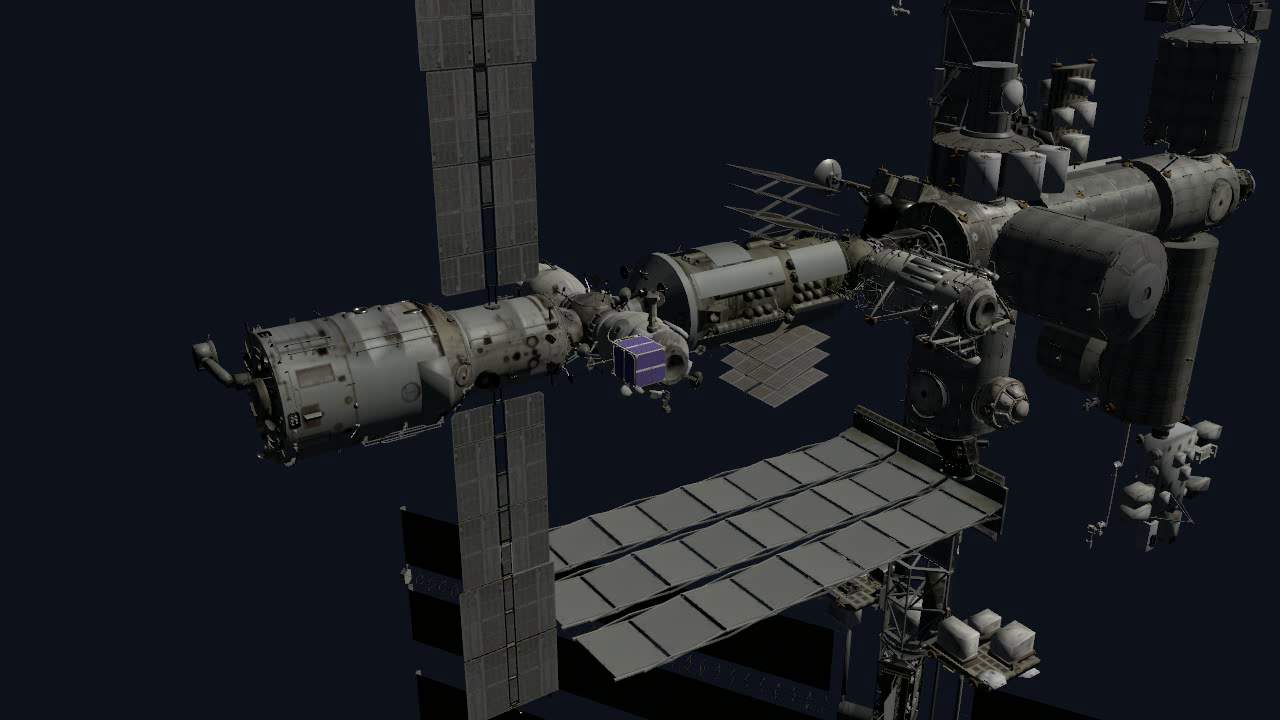
\includegraphics[width=\columnwidth]{figures/gazebo_validation/full_preview_360.png}
  \caption{ROS~2/Gazebo integration placeholder based on an archived infrastructure smoke frame. The ISS and chaser rendering confirms model loading and visualization bridging only; it predates the proposed graph policy and is not used as performance evidence. Before submission, this frame should be replaced by the Jazzy closed-loop SOOA replay with planned and executed paths and the corresponding tracking and safety records.}
  \label{fig:ros-placeholder}
\end{figure}

\section{Results}
\label{sec:results}

\subsection{Primary Coverage--Effort Comparison}

The complete graph policy reaches 98.33\% inspectable coverage with 18 SOOAs and \unit{19.47}{m/s} cumulative $\Delta v$. The two-stage incumbent reaches the same coverage with 21 SOOAs and \unit{21.59}{m/s}. The returned policy therefore removes three actions and reduces $\Delta v$ by 9.85\% while preserving \unit{9.91}{m} sampled clearance and a positive \unit{1.51}{m} passive-drift margin. Figure~\ref{fig:adp-primary} places this result beside local baselines and shows action count directly rather than using marker area.

\begin{figure}[t]
  \centering
  
\includegraphics[width=\columnwidth]{figures/high_coverage/adp_primary_tradeoff.pdf}
  \caption{Primary saved-result comparison. Position gives final inspectable coverage and cumulative $\Delta v$; annotations give selected action count, and the dashed line marks the 98\% stop target. Circles pass every enabled trajectory and passive-drift audit, whereas X markers fail at least one audit.}
  \label{fig:adp-primary}
\end{figure}

\begin{table*}[t]
  \centering
  \caption{Primary 180-target benchmark. The feasibility column includes the enabled \unit{300}{s} passive-drift audit.}
  \label{tab:method-results}
  \renewcommand{\arraystretch}{1.05}
  \setlength{\tabcolsep}{4.2pt}
  \scriptsize
  \begin{tabular}{@{}lrrrrrrrr@{}}
    \toprule
    Method & $C$ (\%) & SOOAs & $\Delta v$ (m/s) & Peak $u$ (m/s$^2$) & $d_{\min}$ (m) & $\rho_{\min}$ (m) & Plan (s) & Feas. \\
    \midrule
    Complete graph policy & 98.33 & 18 & 19.47 & 0.0385 & 9.91 & 1.51 & 339.92 & Yes \\
    Two-stage incumbent & 98.33 & 21 & 21.59 & 0.0388 & 9.91 & 1.51 & 6.05 & Yes \\
    Coverage greedy & 98.33 & 18 & 49.75 & 0.0849 & $-1.89$ & $-3.43$ & 5.35 & No \\
    Safe coverage & 98.33 & 20 & 45.37 & 0.0581 & 0.89 & $-2.40$ & 6.04 & No \\
    Fuel greedy & 96.67 & 36 & 24.29 & 0.0368 & 0.14 & $-1.99$ & 10.85 & No \\
    \bottomrule
  \end{tabular}
\end{table*}

\subsection{Primary Trajectory Case Study}

Figure~\ref{fig:primary-trajectory} exposes the route-level change hidden by the aggregate statistics. Both methods start from $\mathbf x_0=[0,-35,10,0,0,0]^{\mathsf T}$ and share their first four observation poses. The returned route then reorders the remaining common poses and omits three incumbent-only poses, reaching 98.33\% coverage after 18 rather than 21 SOOAs. This shorter audited sequence reduces cumulative $\Delta v$ from 21.59 to \unit{19.47}{m/s}; both routes retain the same reported \unit{9.91}{m} minimum sampled clearance and \unit{1.51}{m} minimum passive-drift margin. The component study below identifies this returned route with safeguarded local sequence improvement, not with a critic-only policy.

\begin{figure}[t]
  \centering
  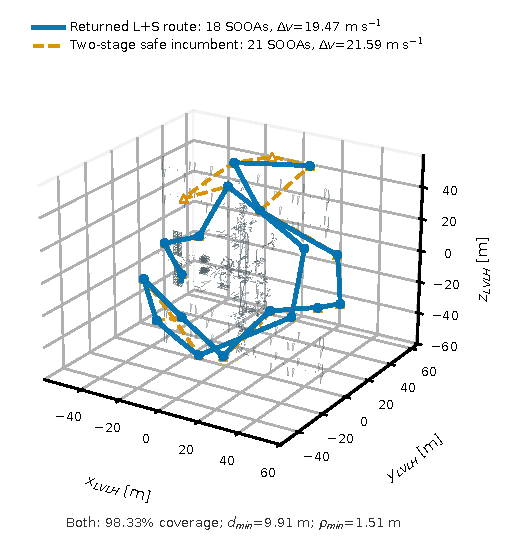
\includegraphics[width=\columnwidth]{figures/high_coverage/primary_trajectory_case_study.pdf}
  \caption{Primary saved-trajectory case study in the LVLH frame. The solid blue curve is the returned route, which is identical to the L+S component result; the dashed gold curve is the two-stage incumbent. Circles and triangles mark terminal observation poses, the green star marks the common initial position, and X markers show the final endpoints. The station mesh provides geometric context; every trajectory sample is loaded from the archived HCW results rather than recomputed during plotting.}
  \label{fig:primary-trajectory}
\end{figure}

\subsection{Component Attribution and Computational Cost}

Table~\ref{tab:method-results} changes the interpretation of the local baselines once passive drift is included in the common feasibility flag. Safe coverage reaches 98.33\% without an instantaneous collision, yet its worst passive margin is \unit{-2.40}{m}; fuel greedy has the same failure and also misses the 98\% stop target. Coverage greedy violates the input, instantaneous-clearance, and passive-drift checks. The complete graph policy is therefore compared with the two-stage incumbent as the only other primary method that both reaches 98\% and passes every enabled audit.

Figure~\ref{fig:adp-components} reports matched cold-cache component runs rather than candidates extracted after executing the complete algorithm. Critic-only planning C nearly doubles incumbent $\Delta v$, from \unit{21.59}{m/s} to \unit{42.86}{m/s}, and increases the action count from 21 to 26. Adding the safeguard S restores the incumbent exactly but requires \unit{278.99}{s}. Rollout with the safeguard R+S reduces $\Delta v$ to \unit{20.92}{m/s} with 20 actions, whereas local search with the safeguard L+S reaches \unit{19.47}{m/s} with 18 actions. Adding critic and rollout to L does not change that route.

\begin{figure}[t]
  \centering
  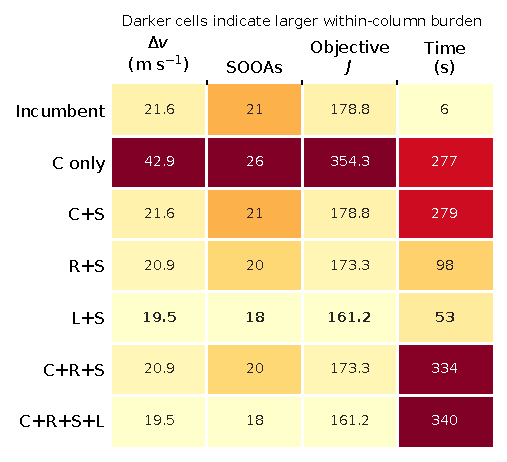
\includegraphics[width=\columnwidth]{figures/high_coverage/adp_component_ablation.pdf}
  \caption{Decision matrix for the matched component ablation. C is critic training and lookahead, R is one-step rollout, S is the incumbent safeguard, and L is audited reversal search. Every variant reaches 98.33\% coverage and passes the enabled audits. Cells report raw values; color is normalized independently within each column, with darker cells indicating a larger burden.}
  \label{fig:adp-components}
\end{figure}

The full C+R+S+L method takes \unit{339.92}{s}, 6.44 times the \unit{52.81}{s} used by L+S, despite returning the same route and objective. C+R+S also reproduces R+S while increasing planning time from \unit{97.64}{s} to \unit{334.11}{s}. Thus local sequence improvement is the source of the primary-case gain, and the critic produces no solution-quality improvement in this deterministic primary case. The complete method is an offline diagnostic architecture in its present implementation, not a real-time planner.

\subsection{Reduced-Graph Certification}

Across the tested 8-, 10-, and 12-node families, safeguarded rollout matches the exact Bellman cost for every seed, giving zero reported optimality gap. Figure~\ref{fig:adp-oracle} also reports the number of expanded Bellman states, which grows with graph size even under the modest seven-action horizon. Exploration seed changes the learned critic but not the deterministic graph optimum. These cases verify the state recursion and returned graph objective; they do not establish optimality on the 96-node primary graph.

\begin{figure}[t]
  \centering
  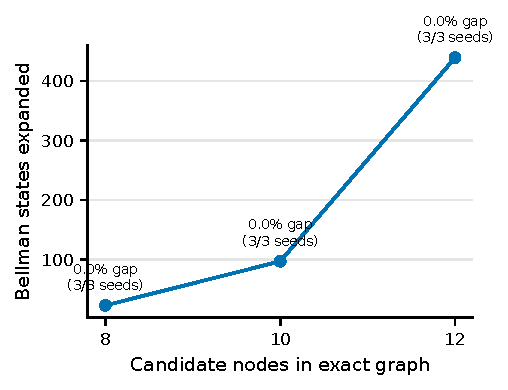
\includegraphics[width=\columnwidth]{figures/high_coverage/adp_oracle_gap.pdf}
  \caption{Exact-oracle verification on reduced graphs. Vertical position is the number of Bellman states expanded; each point is annotated with the returned-policy cost gap to the exact optimum. Multiple seeds test the learned proposal while leaving the deterministic exact problem unchanged.}
  \label{fig:adp-oracle}
\end{figure}

\subsection{Initial-State Stress Tests}

Figure~\ref{fig:adp-initial} separates effort from passive feasibility. At IC-0, policy improvement reduces $\Delta v$ from 21.59 to \unit{19.47}{m/s}; both policies retain a positive passive margin. At IC-1, the two-stage incumbent is cheaper at \unit{23.09}{m/s} but has $\rho_{\min}=\unit{-2.45}{m}$. The shield rejects that completion, and the complete graph policy instead returns a \unit{37.12}{m/s} route with $\rho_{\min}=\unit{4.12}{m}$. At IC-2, both policies have $\rho_{\min}=\unit{6.86}{m}$, and one-step rollout gives a small reduction from 20.19 to \unit{20.10}{m/s}. The higher effort at IC-1 is therefore the cost of satisfying the enabled audit, not a performance improvement in fuel.

\begin{figure}[t]
  \centering
  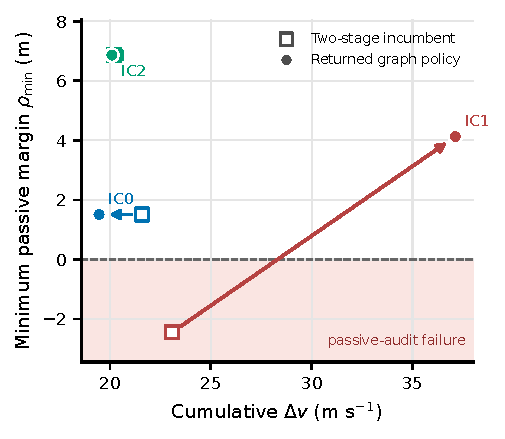
\includegraphics[width=\columnwidth]{figures/high_coverage/adp_initial_condition.pdf}
  \caption{Connected safety--effort comparison across initial conditions. Each arrow starts at the two-stage incumbent and ends at the returned graph policy. The horizontal coordinate is cumulative $\Delta v$, the vertical coordinate is minimum passive-drift margin, and the shaded region fails the enabled passive audit. IC-0, IC-1, and IC-2 are defined explicitly in Section~\ref{sec:simulation}.}
  \label{fig:adp-initial}
\end{figure}

The three cases are deterministic stress tests rather than a statistical robustness guarantee. They show that the base policy can remain adequate, can be improved, or can become passive-unsafe as the start changes. The shield and safeguard respond to these cases differently: no-degradation applies only when the supplied base policy is itself coverage-satisfying and shield-feasible.

\subsection{Critic and Lookahead Compute Tradeoff}

Figure~\ref{fig:adp-compute} shows that additional training is not monotonically beneficial on the truncated 48-node graph. With no Monte Carlo fitting and depth 1, the initial hand-scaled features reach 94.44\% weighted surface coverage in \unit{60.77}{s}. Twenty episodes with depth 2 cross the 95\% target, reaching 95.56\% in \unit{83.98}{s}. Eighty episodes at the same depth reduce the partial-path objective but terminate at 92.22\%, despite a smaller mean absolute training error. This behavior is consistent with value approximation error and distribution shift; it is why Algorithm~\ref{alg:safe-graph-api} retains a success-aware incumbent rather than accepting the lowest predicted cost.

\begin{figure}[t]
  \centering
  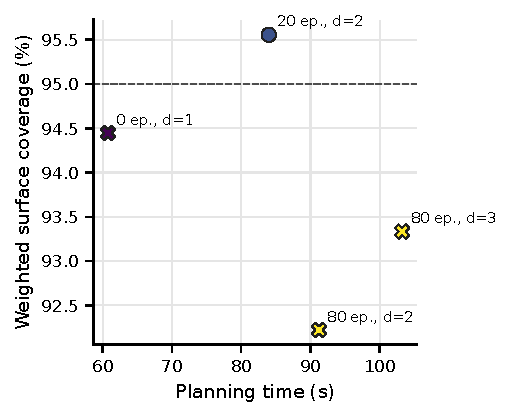
\includegraphics[width=\columnwidth]{figures/high_coverage/adp_compute_tradeoff.pdf}
  \caption{Compute ablation on the 90-target, 48-node graph. Position gives cold-cache planning time and weighted surface coverage; annotations give training episodes and lookahead depth. Circles reach the 95\% graph goal and X markers do not.}
  \label{fig:adp-compute}
\end{figure}

The depth-3 case tests whether more online search repairs the critic. Planning time rises from \unit{91.23}{s} at depth 2 to \unit{103.25}{s}, but coverage reaches only 93.33\%; the additional expansion does not restore the target. These results rule out a blanket convergence claim for the linear critic and motivate future fitted-value or graph-neural approximators with validation on held-out initial states.

\subsection{Cross-Result Synthesis}

The results separate six questions that a final-coverage number would collapse. Figure~\ref{fig:adp-primary} asks whether a successful shield-feasible policy reduces effort and action count, while Fig.~\ref{fig:primary-trajectory} shows how the selected sequence changes in the primary case. Figure~\ref{fig:adp-components} identifies which enabled component produces that gain. Figure~\ref{fig:adp-oracle} checks the finite-state implementation against exact Bellman recursion. Figure~\ref{fig:adp-initial} tests whether a low-effort incumbent remains passively safe when the start changes, and Fig.~\ref{fig:adp-compute} exposes the accuracy--runtime tradeoff of approximate values. Together they support a bounded conclusion: safeguarded local graph improvement can improve a feasible incumbent, and the broader architecture can replace an unsafe incumbent under the stated HCW and sampled-audit model; critic training alone is neither sufficient nor monotonically beneficial.

\section{Discussion}
\label{sec:discussion}

The candidate-node MDP strengthens the formulation beyond static next-best-view selection because covered area, current terminal node, selected observations, and remaining budget enter the decision state explicitly. Proposition~\ref{prop:markov-sufficiency} establishes Markov sufficiency under the fixed-graph assumptions, and the reduced-oracle results test the implementation of that recursion on exhaustible cases. On the primary graph, however, the critic-only sequence is substantially worse than the incumbent, and the complete result is reproduced by safeguarded local search. The demonstrated primary advantage therefore comes from the safety-shielded graph representation and audited sequence improvement, not from an unsupported claim that reinforcement learning discovers a superior policy.

The passive audit changes which comparisons are meaningful. A transfer can satisfy input and instantaneous clearance while its uncontrolled continuation enters the protected region. Treating `passive safe' as a separate diagnostic but excluding it from the common feasibility flag would make a low-effort unsafe tour appear superior. The corrected evaluation requires every method to pass the same enabled audit. IC-1 then shows the intended behavior: the complete graph policy accepts greater effort to replace a passive-unsafe incumbent. Because the primary ablation finds no critic benefit, this stress case supports only a conditional role for learned proposals when the base completion is inadmissible.

The primary cost reduction is empirical and library-conditional. Audited reversal improves the supplied base sequence, one-step rollout provides a smaller improvement, and the critic-only candidate degrades it. The 6.44-fold runtime gap between the complete method and L+S further argues against deploying the full stack without a case where the critic adds value. Different candidate densities, motion-primitive families, or critic features may change that attribution. The no-degradation theorem applies only to the shared graph objective and only when the base sequence is feasible on the same finite graph; it guarantees neither lower physical $\Delta v$ in every case, continuous-space optimality, nor improvement when the base policy fails the shield.

The relation to formation-based observation is similarly complementary. Near-natural relative ellipses and closed-loop formation control around a rotating station can provide lower-effort motion structure and stronger stability analysis \cite{zhou2026formation}. OrbInspect instead resolves which surface regions are visible, how prescribed observations are credited, and which observation should follow the current state. A useful synthesis would generate SOOA candidates from near-natural orbit families, then select among them using the present coverage and camera model. This could reduce transfer effort while preserving explicit target-level inspection accounting.

The safety evidence remains limited to the stated model. HCW translation assumes a circular chief and a fixed LVLH target. Clearance is checked on sampled trajectories against deterministic station primitives, and passive drift is audited only over a prescribed horizon. There is no closed-loop proof under navigation error, target rotation, delayed commands, actuator uncertainty, or between-sample collision. The exact oracle certifies only the exhausted reduced graphs, and the full solver has no continuous-space optimality guarantee.

The camera evidence has comparable boundaries. The visibility model includes range, field of view, incidence, and mesh occlusion, but the offline graph credits a prescribed terminal observation rather than simulating exposure interruption or closed-loop dwell. Illumination, blur, plume contamination, camera slew, and detailed attitude dynamics are omitted. ROS~2 and Gazebo replay remain implementation work and are not treated as validation in the present manuscript.

A flight-oriented development path should first accelerate cached passive audits and batched edge evaluation, since the primary planning-time penalty is large. A held-out validation protocol and fitted or graph-structured critic should then replace the present linear Monte Carlo approximation. Uncertainty-inflated keep-out volumes, camera-slew and illumination constraints, plume restrictions, navigation error, and a rotating body frame should follow. Higher-fidelity propagation, including an optional Basilisk backend, can finally be introduced while retaining HCW as a transparent regression reference.

\section{Conclusion}
\label{sec:conclusion}

This paper formulated orbital inspection as safety-shielded sequential selection of finite-duration observable orbital arcs. The Markov state retains the current candidate node, covered targets, selected nodes, and remaining budget; critic-guided lookahead, rollout, and local search propose decisions, while an HCW shield and audited incumbent control feasibility and degradation. On the primary ISS graph, the returned policy reaches 98.33\% coverage with 18 actions and \unit{19.47}{m/s} cumulative $\Delta v$, a 9.85\% reduction relative to the two-stage base tour at the same coverage and safety margins. A matched ablation shows that safeguarded local search reproduces this result in \unit{52.81}{s}; the full method takes \unit{339.92}{s}, and critic-only planning is worse than the incumbent. Reduced graphs match the exact Bellman optimum, and the IC-1 case shows why passive-drift feasibility must be evaluated alongside instantaneous clearance.

The evidence also defines the boundary of the contribution. The learned critic does not produce the primary gain, additional training is not monotonically beneficial on a truncated graph, and the full-stack planning-time overhead is substantial. Its role is presently conditional: it supplies an alternative in the tested IC-1 case when the incumbent is rejected, but its superiority is not demonstrated. Exact optimality is limited to exhausted reduced graphs; audit preservation is limited to the deterministic sampled HCW, geometry, and passive horizon. The result is therefore a transparent safety-shielded finite-graph policy-improvement framework, not a flight-certified, continuously safe, or continuously optimal solution.

\bibliographystyle{IEEEtran}
\bibliography{references}

\begin{IEEEbiography}
    [{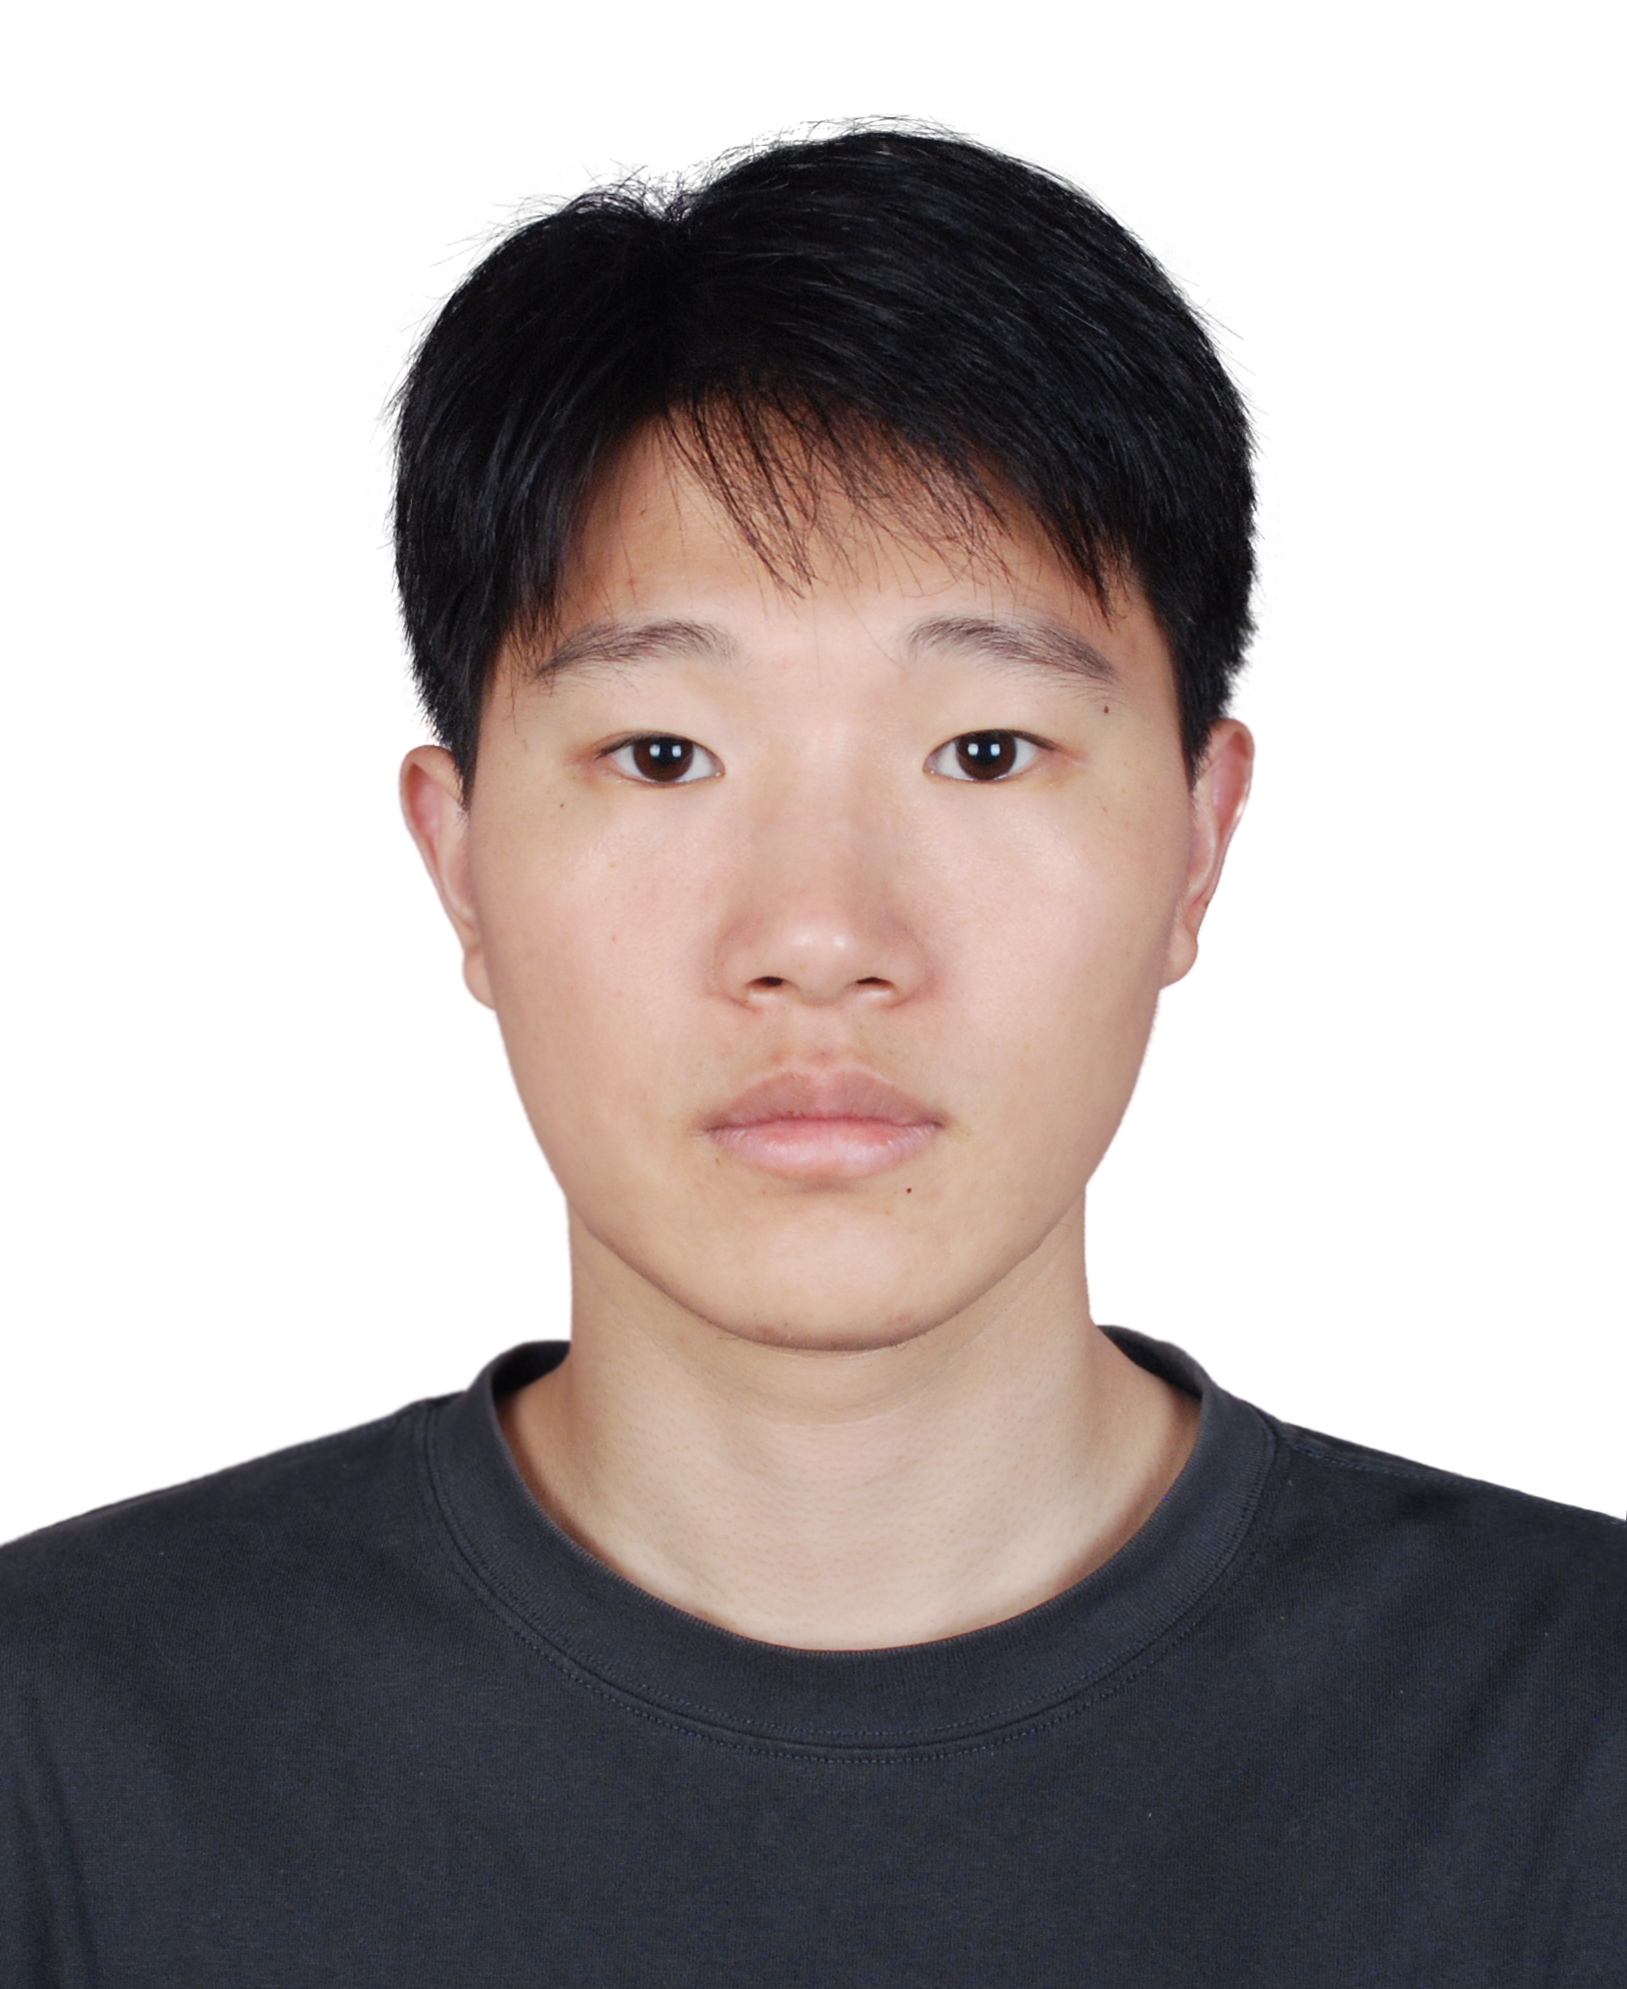
\includegraphics[width=1in,height=1.25in,clip,keepaspectratio]{figures/authors/trg.jpg}}]{Rugang Tang} received the B.Eng. degree in aircraft design and engineering from Northwestern Polytechnical University, Xi'an, China, in 2020. He is pursuing the Ph.D. degree in aircraft design with the Department of Aeronautical and Aviation Engineering, The Hong Kong Polytechnic University, Hong Kong. His research interests include multi-agent and nonlinear systems, reach-avoid differential graphical games, and approximate dynamic programming.
\end{IEEEbiography}

\begin{IEEEbiography}[{
\includegraphics[width=1in,height=1.25in,clip,keepaspectratio]{figures/authors/nx.pdf}}]{Xin Ning} received the B.Eng., M.Eng., and Ph.D. degrees from Northwestern Polytechnical University, Xi'an, China, in 2004, 2007, and 2011, respectively. He is a Professor and Vice Dean of the School of Astronautics at Northwestern Polytechnical University and was a visiting scholar at the University of Calgary. His research interests include aerospace flight dynamics, navigation, guidance and control, spacecraft on-orbit servicing, trajectory planning, intelligent optimization, nonlinear systems, and modeling.
\end{IEEEbiography}

\begin{IEEEbiography}
    [{
\includegraphics[width=1in,height=1.25in,clip,keepaspectratio]{figures/authors/CYW.png}}]{Chih-yung Wen} received the B.S. degree from National Taiwan University in 1986 and the M.S. and Ph.D. degrees from the California Institute of Technology in 1989 and 1994, respectively. He is Head and Chair Professor of Aeronautical Engineering with the Department of Aeronautical and Aviation Engineering, The Hong Kong Polytechnic University, and Associate Director of its Research Institute for Sports Science and Technology. His professional activities span mechanical and aerospace engineering.
\end{IEEEbiography}

\end{document}
